\subsection{Safecode}

\subsubsection{Writing Operation}
\label{sec:WRITING_OPERATION}

In order to be able to check the introduced password, we will program it into a Random Access Memory (RAM), in particular a 6116 CMOS Static one so as to be able to read it later on. To do this, we will use a GAL. In this case, the clock (CLK) and the BCD signal from the KEYPAD GAL (SIG) will be its inputs. In order for the RAM to work properly, it requires the SAFECODE GAL to have as output a Chip Select signal (CS\_\_), an Address signal (A), and the BCD (D\_\_).\medskip

As the programmable chip acts as a FSM, it will also have as output a representation of its current state, which will be later used to command other GAL devices. It should be noted that due to the fact that the RAM IC will be commanded by different GALs, we have added resistors between the output of the GAL and the control pins of the RAM so as to avoid short circuits. We can clearly see this in the following picture:

\begin{figure}[H]
    \centering
    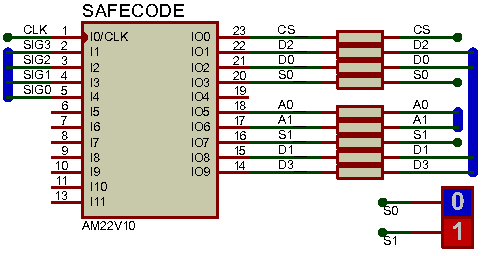
\includegraphics[scale = 1]{Graphics/SAFECODE/SAFECODE_PROTEUS.PDF}
    \caption{Proteus Subassembly of Safecode}
    \label{fig:SAFECODE_PROTEUS}
\end{figure}


\medskip
The memory device will start storing data when the Write Enable ($\overline{WE}$) signal and the Chip Select ($\overline{CS}$) are pulled LOW by the GAL. A timing diagram is attached:\medskip

\begin{figure}[H]
    \centering
    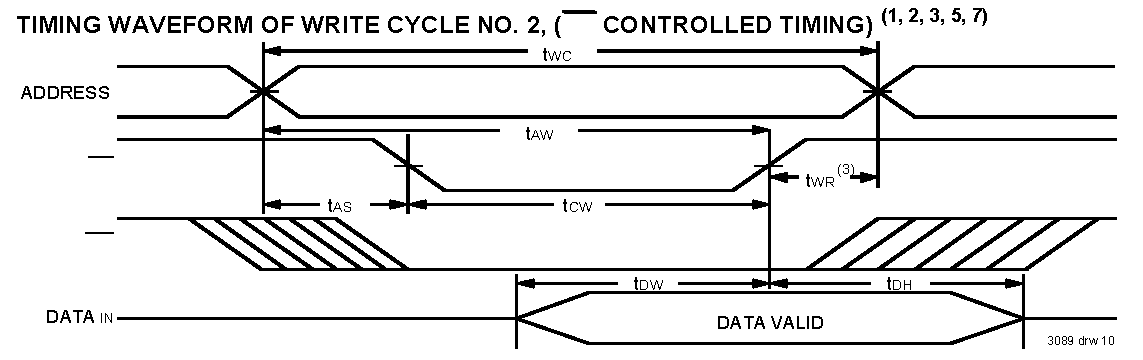
\includegraphics[scale = 0.60]{Graphics/RAM/6116.pdf}
    \caption{6116 RAM Write Cycle}
    \label{fig:6116}
\end{figure}


The general truth table of this specific RAM, though it is mostly the same for most RAM chips, can be found in \textbf{Table} \textbf{\ref{table: RAM_MODES}} \medskip

Now we will discuss the different states that we have defined in our FSM. As per before, the full code will be attached as well.

\subsubsection{FSM States Overview}

    \hspace{0.4cm}
    \bm{$Q_0$}
\medskip

At rest, the system must start at Address "00", and the $\overline{CS}$ signal must be HIGH because it is active when it is LOW. Once the $*$ button is pressed, system transitions to $Q_1$ state.

\medskip
    \bm{$Q_1$}
\medskip

The $\overline{CS}$ signal changes to a LOW level, and the RAM device is in the “ready to write” State $Q_1$. This means that from now on, Address number $00$ is ready to be overwritten by the character we introduce with the keypad. 

\medskip
When introducing a new character with the keypad, the $*$ will make the system stay at $Q_1$,  the \textit{\#} character will make the system to return to $Q_0$, and any other character will make the system change to State $Q_2$. \medskip

\bm{$Q_2$} \textbf{\&} \bm{$Q_3 \textit{\textbf{ and return to }} Q_0$}\medskip

In state $Q_2$, the character previously introduced is written on the address $00$.

\medskip
Now, there are two options: to keep writing on the memory, or to stop writing.


\begin{itemize}
    \item In order to keep writing, any key pressed but \textit{\#} and the same key, will transition the system to state $Q_3$, where the system jumps to the next Address (where the next character will be kept), and the writing loop starts again at \textit{$Q_1$}.
    
    \item In order to stop, the  \textit{\#} button is pressed, and the system returns to state \textit{$Q_0$}, meaning that  the Address is reset to $00$, and the writing operation ends.
\end{itemize}

\clearpage

To illustrate the different states and the transitions between them we have included the following diagram:

\begin{figure}[H]
    \centering
    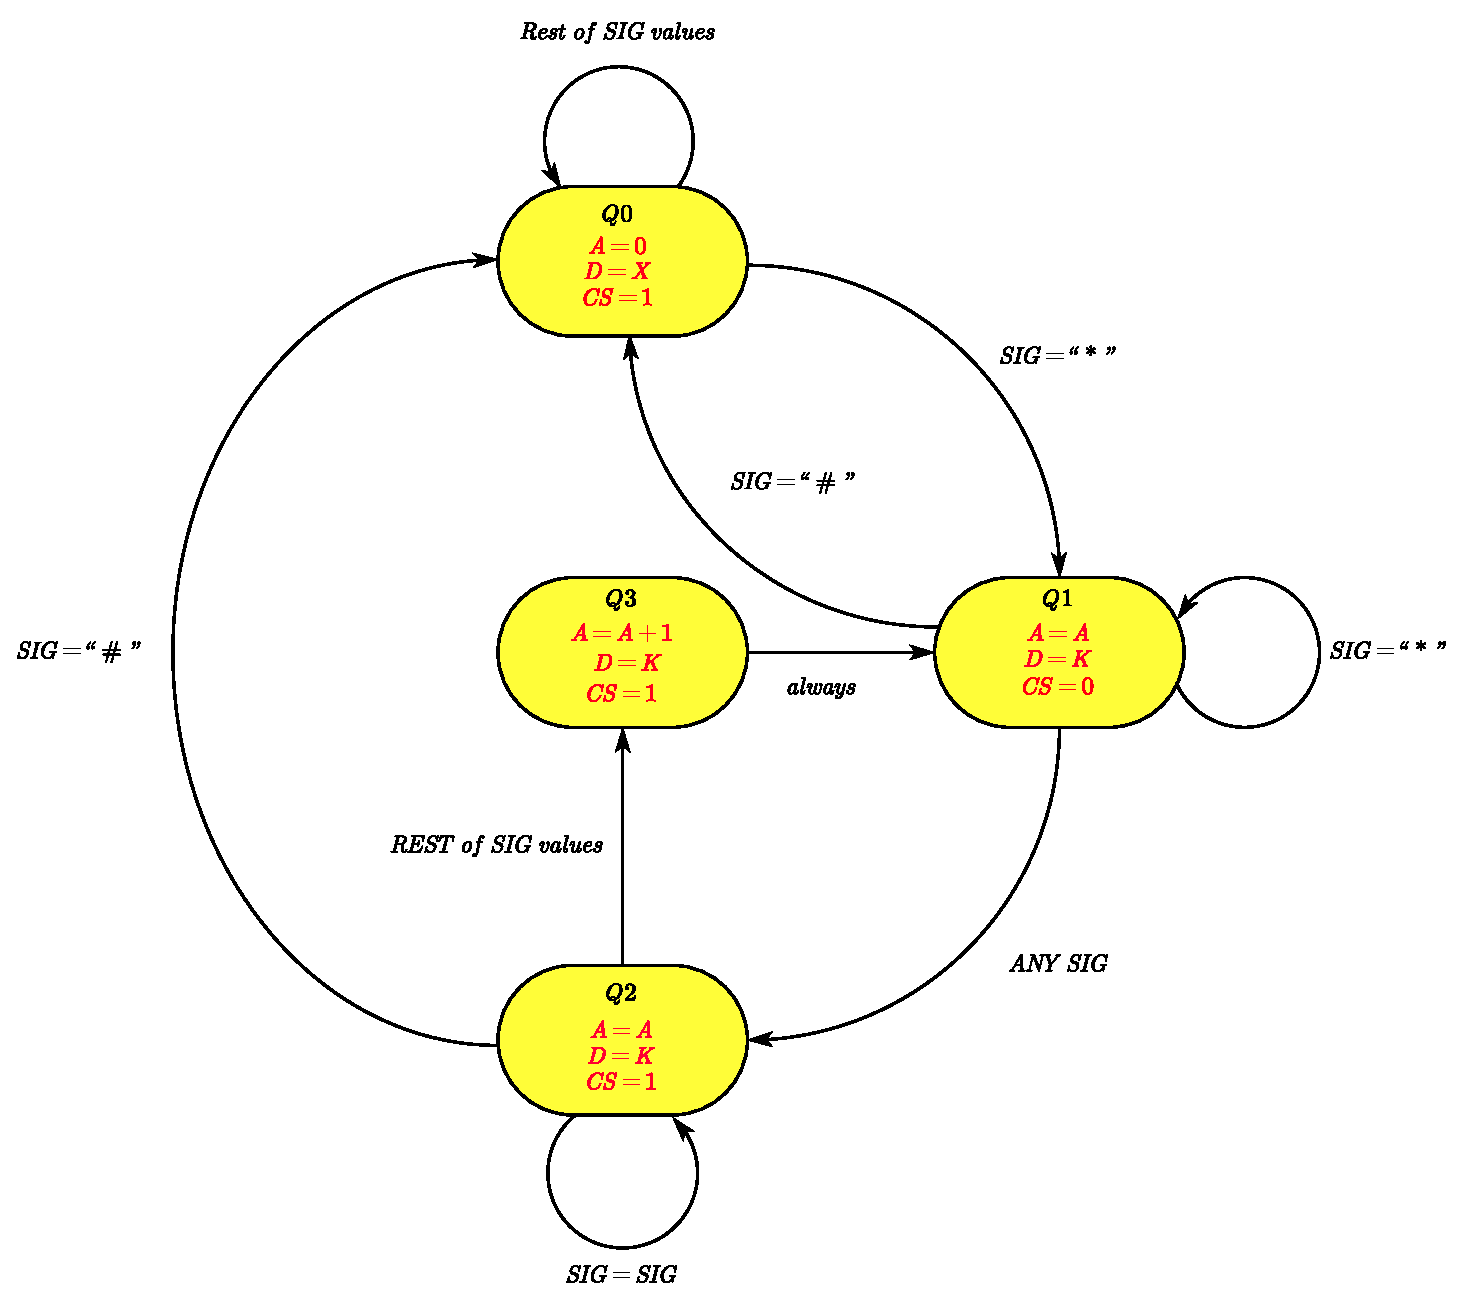
\includegraphics[scale = 0.55]{Graphics/SAFECODE/SAFECODE.pdf}
    \caption{Safecode FSM}
    \label{fig:SAFECODE_FSM}
\end{figure}

The VHDL code for this GAL can be found below:

\inputcode{Code/SAFECODE.vhd}
            

